\section{Time-of-Flight Detectors}\label{sec:clas.tof}

Accurate measurement of the speed of the final state particles, as discussed in Sec.~\ref{sec:data.calib.systems}, is challenging. Because of their relatively low momentum, typically 1--2~GeV, the particles travel slow enough that the time it takes them to reach the time-of-flight\cite{clas.tof} (\abbr{TOF}) counters is significant. It is thanks to the fine timing resolution of \abbr{CLAS} that enables the \abbr{TOF} to provide the particle identification used in this analysis.

The \abbr{TOF} consists of six outer shells, one of which is shown in Fig.~\ref{fig:clas.tof.paddles}, of 57 scintillator paddles. The paddles are grouped physically into four \emph{panels}. The paddles are all 5.08~cm (2~inches) thick but are of varying lengths and each has a \abbr{PMT} attached to both ends. This provides close to 100\% efficiency of minimum ionizing particles and a timing resolution of 150--200~ps as discussed in Sec.~\ref{sec:data.calib.systems}. The \abbr{TOF} detector was used in the level 1 trigger (see Sec.~\ref{sec:data.trig}) for \g12 to identify ``prongs'' or track candidates. Also, the \abbr{ADC} signals from the \abbr{TOF} were used to measure the energy deposit of the tracks to assist in particle identification in Sec.~\ref{sec:analysis.tofe}.

\begin{figure}\begin{center}
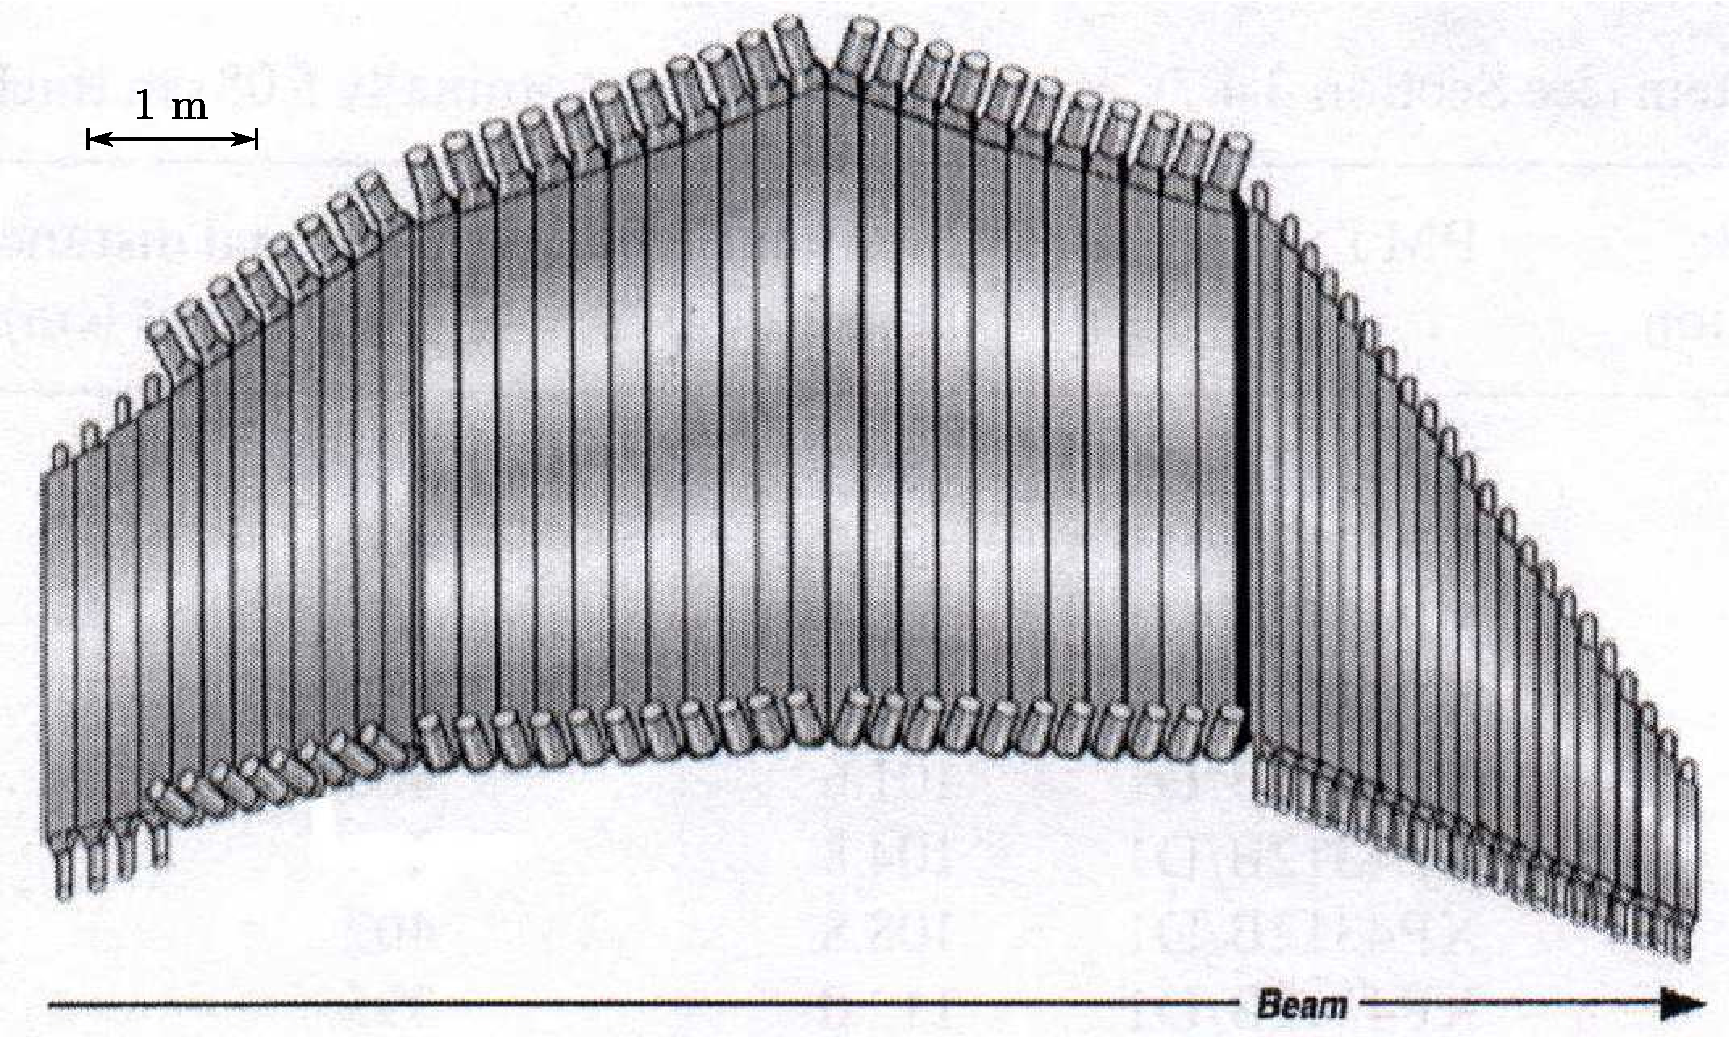
\includegraphics[width=\figwidth]{\figures/hall-b/tof_paddles.pdf}
\caption[Time-of-Flight Paddles]{\label{fig:clas.tof.paddles}Diagram of one sector of the time-of-flight (\abbr{TOF}) paddles. There are 57 scintillator paddles covering the entire acceptance region of the drift-chambers for each sector.}
\end{center}\end{figure}

\begin{figure}\begin{center}
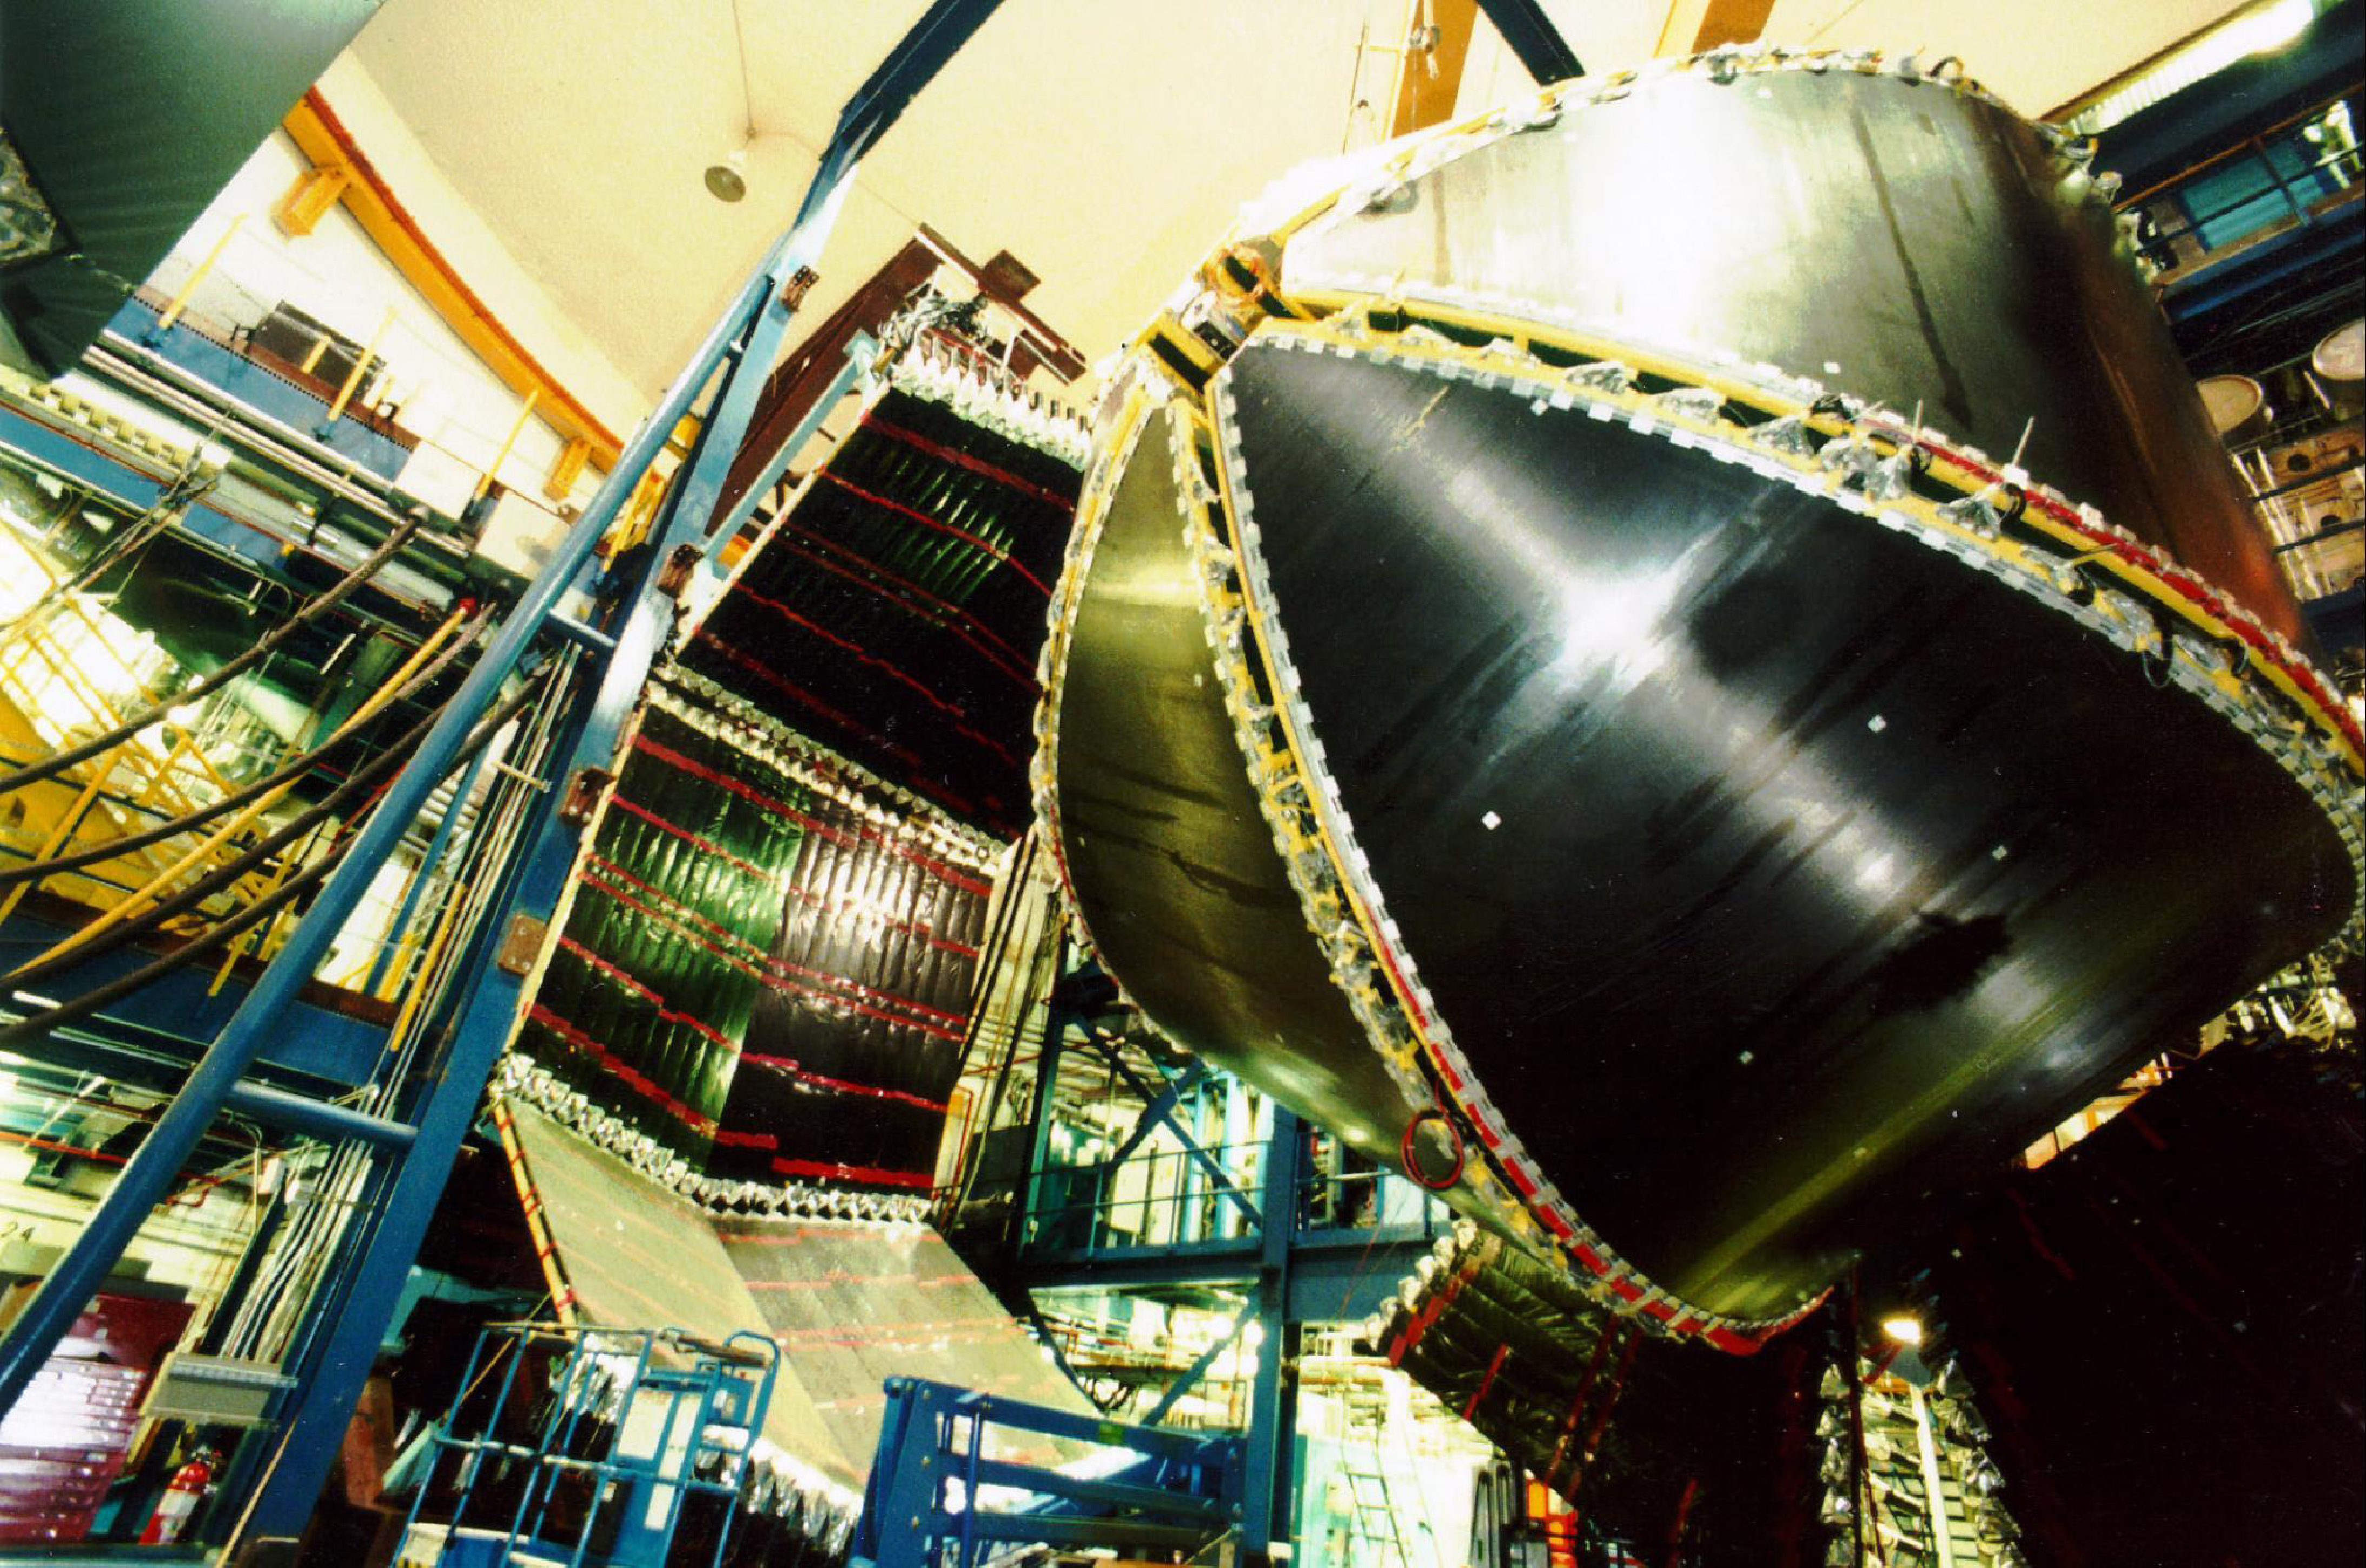
\includegraphics[width=0.8\columnwidth]{\figures/hall-b/clas_detector.pdf}
\caption[\abbr{CLAS} Detector (photograph)]{\label{fig:clas.photo}The \abbr{CLAS} detector during a maintenance period where the time-of-flight ``shell'' (left) was pulled back from the drift-chambers (\abbr{DC}, right). The beam line enters from the lower right on the other side of the \abbr{DC}. The \abbr{TOF} paddles seen are the two center \emph{panels} shown in Fig.~\ref{fig:clas.tof.paddles} for three of the \abbr{CLAS} sectors.}
\end{center}\end{figure}

\begin{figure}\begin{center}
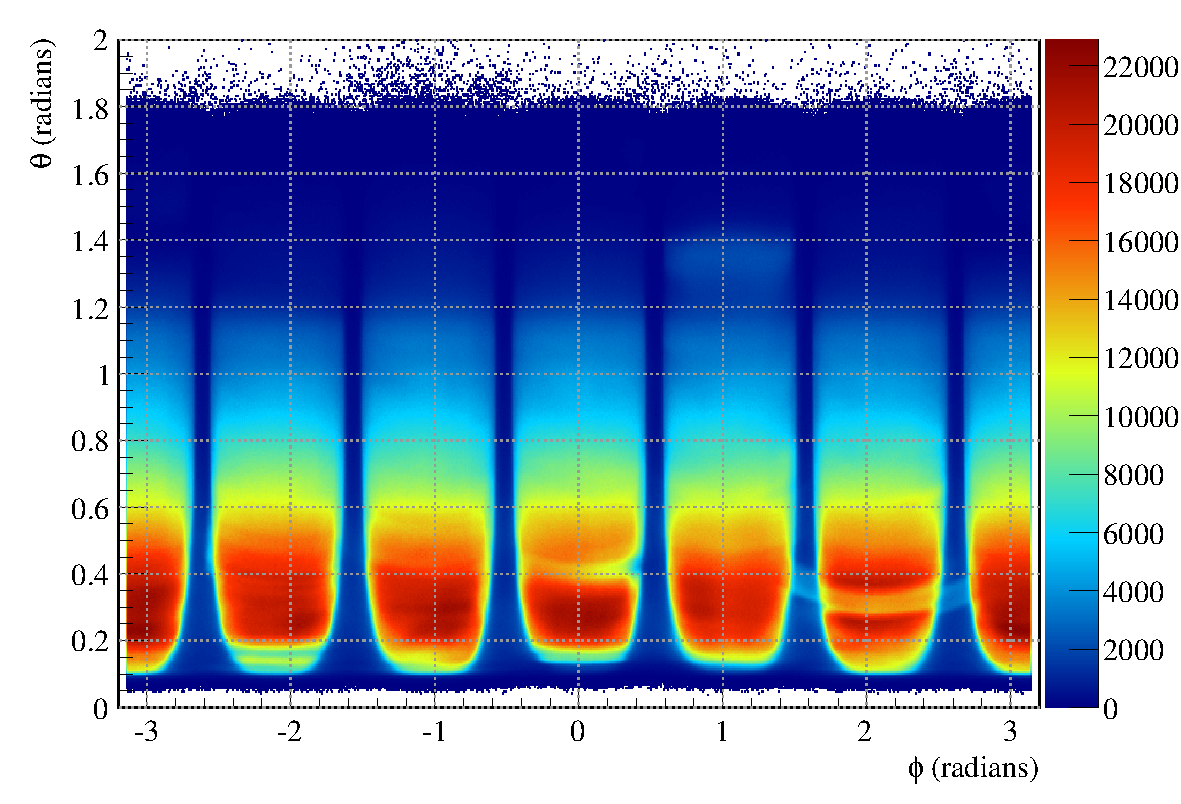
\includegraphics[width=\figwidth]{\figures/reconstruction/coverage_tof.pdf}
\caption[Time-of-Flight Angular Coverage]{\label{fig:clas.tof.coverage}{\coloronline}Angular coverage in the lab frame of the tracks that had an associated time-of-flight hit. This can be interpreted as the total drift-chamber coverage of the \abbr{CLAS} detector.}
\end{center}\end{figure}
